%!TEX TS-program = pdflatex

\documentclass[12pt]{article}
\usepackage{amsfonts, amsmath, amssymb}
\usepackage{dcolumn, multirow}
\usepackage{setspace}
\usepackage{graphicx}
\usepackage{tabularx}
\usepackage{anysize, indentfirst, setspace}
\usepackage{verbatim, rotating, paralist}
\usepackage{latexsym}
\usepackage{amsthm}
\usepackage{parskip}
\usepackage{hyperref}
\usepackage{color}
\usepackage[right=2.5cm, left=2.5cm, top=3.5cm, bottom=3.5cm]{geometry} %right=, left=, top=, bottom=

\title{Estimate the Impact of Opioid Control Policies}
\author{Mid-Semester Project, Practical Data Science 1}
\date{\today}

\begin{document}
\maketitle

\subsection*{Background}

Over the past two decades, the United States has seen a tremendous increase in the use and abuse of prescription opioids, leading not only to a huge rise in opioid addiction, but also a rise in prescription overdose deaths, and increasingly deaths from non-prescription opioids like heroin and fentanyl as people who became addicted to opioids due to prescriptions turn to illegal markets to sustain their addiction.

\begin{figure}[h!]
  \centering
  \caption{Opioid Epidemic}\label{}
  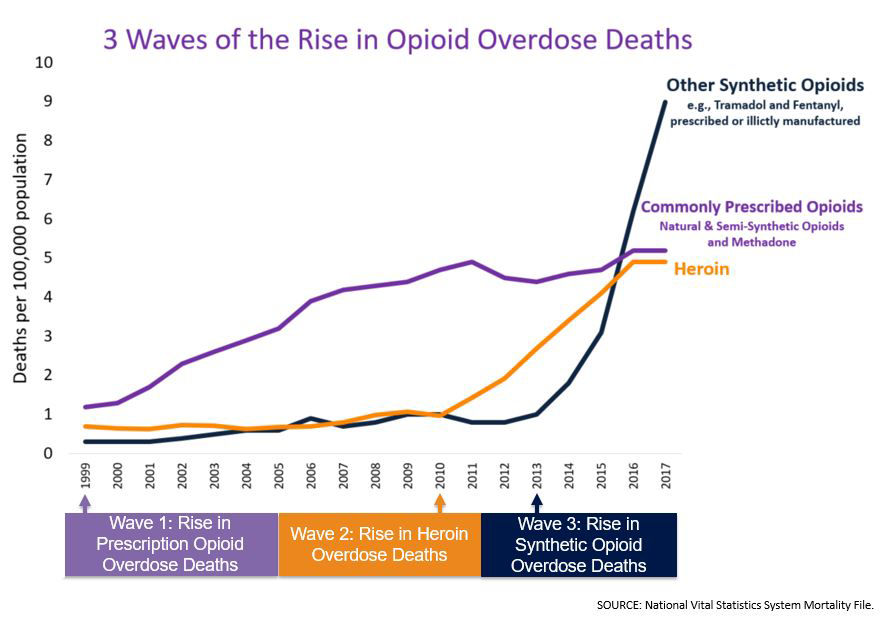
\includegraphics[width=0.6\textwidth]{images/cdc_opioid_stats.png}\\
  \scriptsize{Source: US Centers for Disease Control}
\end{figure}

In this project, we'll be \textbf{estimating the effectiveness of policy interventions} designed to limit the over-prescription of opioids. More specifically, we will attempt to measure the \textbf{effect} of a series of policy changes designed to limited opioid abuse in several US states on (a) opioid drug prescriptions, and (b) mortality from drug overdoses.\footnote{ In particular, we will focus on a Texas regulation that went into effect in January 2007, a Washington regulation that went into effect in January of 2012, and a Florida regulation that went into effect in 2010.}

Our interest in examining mortality as well as opioid prescriptions comes from the fact that while restricting access to opioids may reduce the likelihood that \emph{future} patients will end up addicted to opioids, it may drive already addicted patients to turn to alternative forms of opioids, be those illegally purchased prescription drugs, heroin, or fentanyl. This possibility is deeply troubling because the likelihood of overdosing on these illegal drugs is \emph{much} higher than on (monitored) prescription drugs, as it is impossible for drug users to know the strength of illegal drugs, and because drugs like fentanyl are so potent that as little as 3mg can be lethal.

While our substantive focus is on opioid prescribing regulations, however, it is worth noting that in many ways you can see this as a template for policy evaluations more broadly. This is a specific application of an approach to measuring the impact of a policy, not a novel approach to analyzing opioid regulation.

\subsection*{The Question}

The goal of this project is to answer the following question: what is the effect of opioid drug prescription regulations on

\begin{enumerate}
  \item the volume of opioids prescribed, and
  \item drug overdose deaths.
\end{enumerate}

\subsection*{What An Answer Looks Like}

In developing a data science project, it is good practice to \emph{start} by asking what an answer to your question will look like. Once you know what you are trying to achieve, one can then work backwards to figure out what data will be needed to answer the question, what data manipulations will be required, and how you can divide those tasks among teammates.

In this case, the question we are asking is a \emph{causal question}, meaning that we are interested in understanding the \emph{effect} of one thing on another (i.e. what is the \emph{effect} of X on Y), not just the correlation between two variables.

In a magical, idealized world, the way we would answer a causal question is to create two world: one in which our causal factor (here, a specific policy change) takes place, and one where it does not. Then we can say ``how did things turnout differently for Florida in 2010 (one of our cases) in the world with the policy change \emph{as compared to the world where no policy change took place in Florida in 2010?}''

In the real world, however, we can never actually see both a world with the policy change and a world without the policy change \emph{for the same unit of observation at the same moment in time}. In the language of causal inference, we can never directly observe our \emph{counter factual} (Florida \emph{without} a policy change in 2010) -- we only get to see Florida with the policy change in 2010.\footnote{This is what is referred to as the Fundamental Problem of Causal Inference.}

With that in mind, we have to find a way to \emph{estimate} what we think \emph{would} have happened in Floria had there been no policy change. And this, in a nutshell, is the art of causal inference.

There are many approaches to solving this problem. The one we're most familiar with is randomized drug trials, where we randomly assign people to either take a drug or not take a drug. In these designs, because people are being randomly assigned to take the drug or not, by the law of large numbers we expect the people who take the drug to be, \emph{on average}, the same as the people who don't take the drug. Because of these, we infer that what happens to the people who aren't taking the drug is, \emph{on average}, what \emph{would} have happened to the people do are taking the drug had they not taken the drug. In other words, we think that the non-drug-takers are a good counter-factual for the drug takers.

(If this is making your head spin a little, don't worry -- this stuff is hard, and this is only a \emph{very} quick summary of causal inference. About half of my Spring course will be focused on these ideas.)

But we can't use this strategy for measuring drug policy because we can't randomly assign states to either implement or not implement opioid control measures. With that in mind, we need to come up with different ways of estimating what we think would have happened to Florida had it not passed opioid control measures.

\subsubsection*{Pre-Post Comparison}

One of the most basic strategies, and the one we'll use first, is to compare how things were in Florida right before the policy went into effect to Florida right after the policy went into effect. In doing so, we're assuming that had the opioid policy not gone into effect, Florida in 2011 would have looked more or less like it looked in 2009.

This type of analysis would likely come out with a result that looks something like the plots shown in Figure~\ref{figure_prepost_examples}, where one plot is shown for what a potentially successful policy might look like, and one plot is shown for what an unsuccessful policy might look like.

\begin{figure}[h!]
  \centering
  \caption{Pre-Post Model Figures}\label{figure_prepost_examples}
  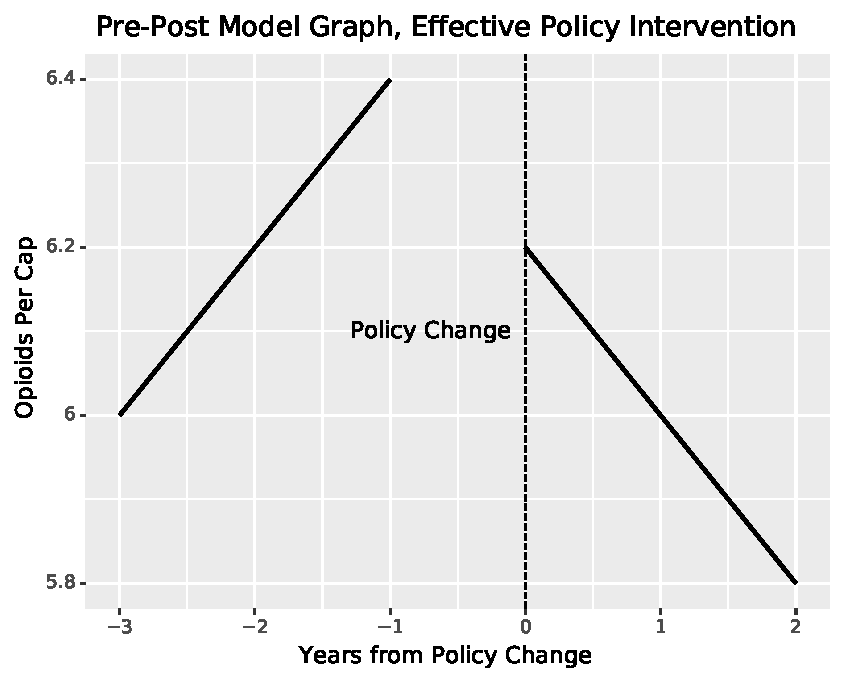
\includegraphics[width=0.5\textwidth]{images/prepost_successful.pdf}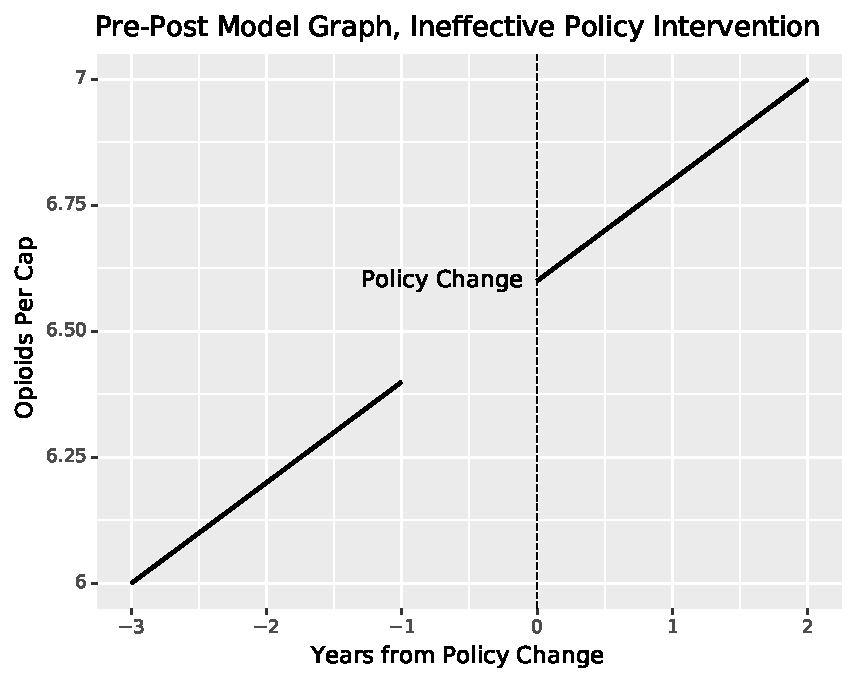
\includegraphics[width=0.5\textwidth]{images/prepost_failed.pdf}
\end{figure}
\pagebreak
\subsubsection*{Difference-in-Difference}

A simple pre-post comparison is a good, simple approach to causal inference, but it is not without its problems.

Suppose, for example, that around 2010 (the same time Florida's policy went into effect) the US Customs service managed to dramatically reduce the importation of fentanyl into the United States. This would likely reduce the amount of overdose deaths throughout the United States, and so if we were just comparing Florida in 2009 to Florida in 2011, we would see a decline in overdose deaths and wrongly attribute that to Florida's policy change.

One strategy for dealing with this is what's called a \emph{difference-in-difference} approach. In simple terms, we don't just compare Florida in 2009 to Florida in 2011; instead, we ask ``were there bigger changes in overdose deaths in Florida between 2009 and 2011 \emph{than in other states that didn't change their opioid policy}?'' If Florida's policy had an effect, then we would expect opioid overdoses in Florida to decrease differently than overdoses in states without a policy change. But if Florida experienced a decline in overdoses because of something that happened nationally (e.g. if US Customs blocked opioid importation), then we'd expect to see overdoses to reduce at the same rate in all states.

In other words, if we see a decline in Florida overdoses, we want to know whether the change we saw in Florida (the ``difference'' from pre-to-post) is larger than the change that occurred in other states over the same period? Or, to map this onto the term ``difference-in-difference,'' if we estimate the \emph{difference} between 2009 and 2011 separately for Florida and states without policy changes, is there a difference in those differences?

This type of analysis would likely come out with a result that looks something like the plots shown in Figure~\ref{figure_diffindiff_examples}, where one plot is shown for what a potentially successful policy might look like, and one plot is shown for what an unsuccessful policy might look like.

\begin{figure}[h!]
  \centering
  \caption{Difference-in-Difference Example Plots}\label{figure_diffindiff_examples}
  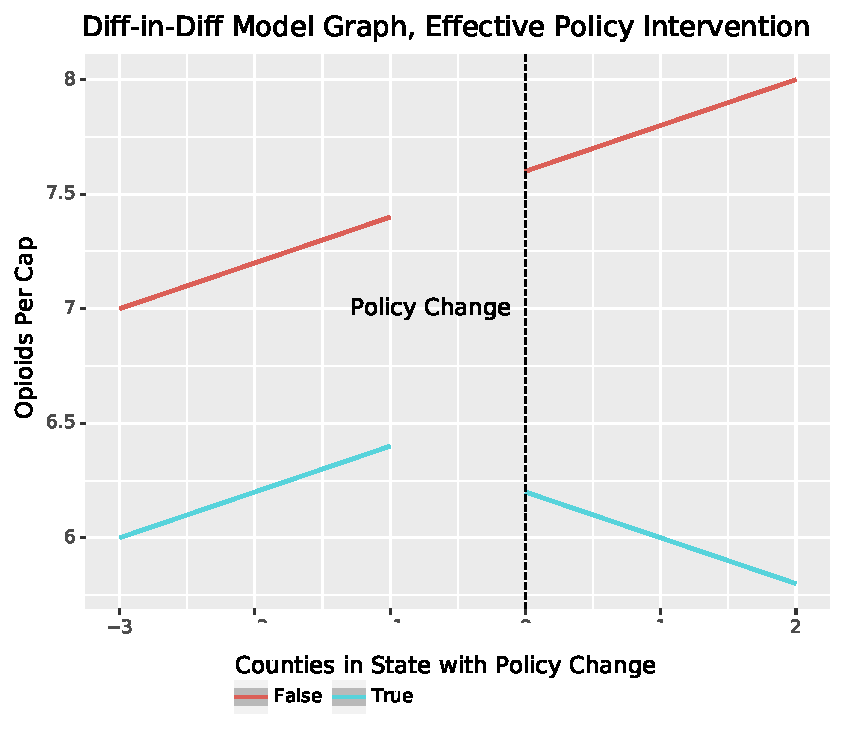
\includegraphics[width=0.5\textwidth]{images/diffindiff_successful.pdf}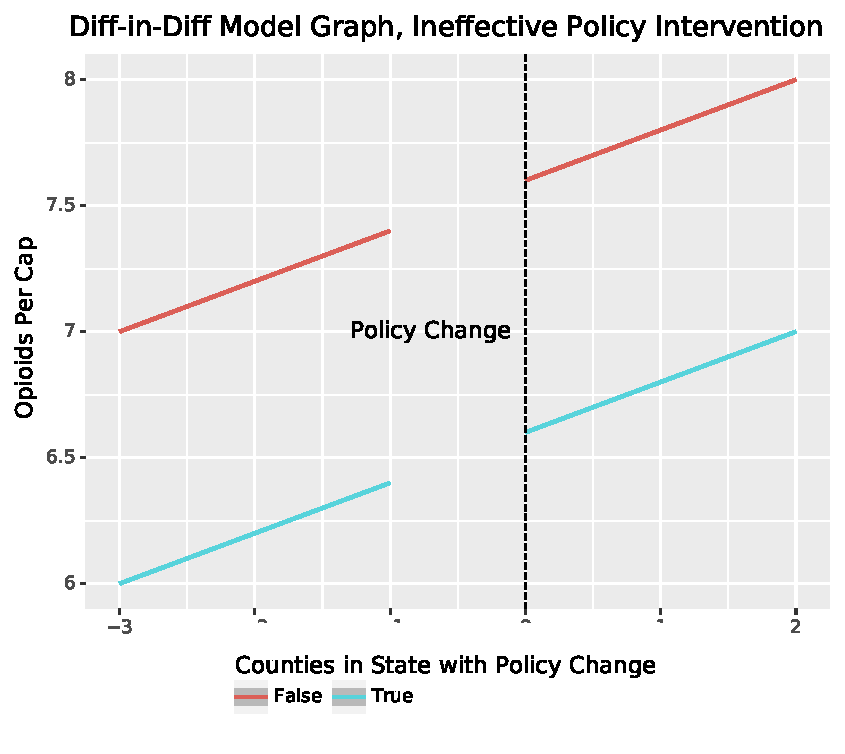
\includegraphics[width=0.5\textwidth]{images/diffindiff_failed.pdf}
\end{figure}

In addition to making this kind of plot, a difference-in-difference can also be estimated statistically using a linear regression model, as detailed in Appendix~\ref{appendix_diffindiff}.

To be clear, difference-in-differences aren't \emph{always} valid. The assumption of a difference-in-difference design is that while our policy-change state (Florida) doesn't have to be the same as our non-policy-change states (everyone else) in \emph{levels}, the two groups do have to exhibit similar \emph{trends} before the policy change being studied. Otherwise, the difference-in-difference may be large even if there's no policy change.

\begin{figure}[h!]
  \centering
  \caption{}\label{figure_diffindiff_nonparallel}
  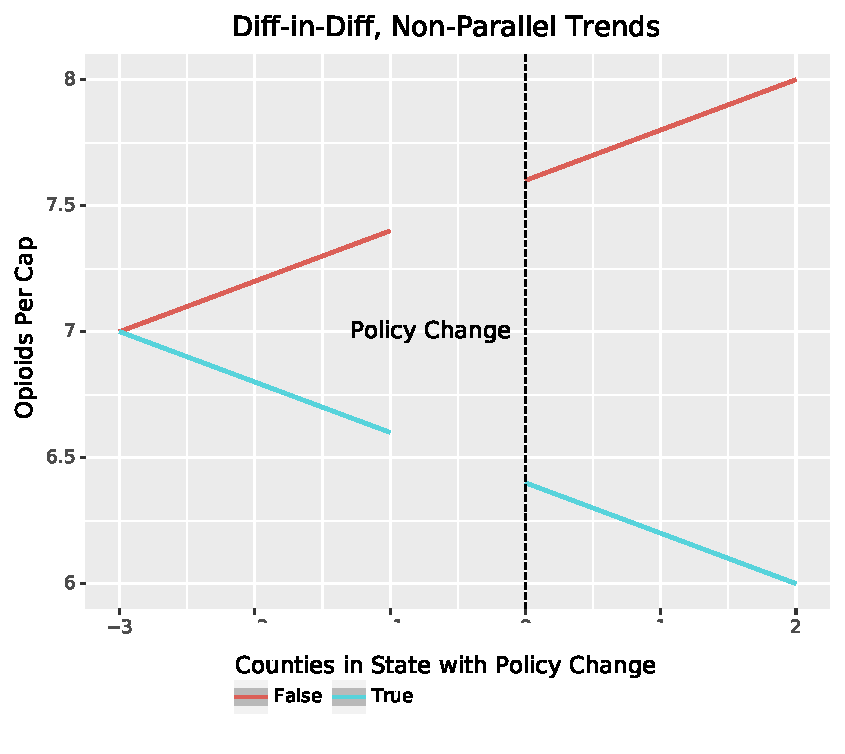
\includegraphics[width=0.7\textwidth]{images/diffindiff_non_parallel.pdf}
\end{figure}


To illustrate, consider Figure~\ref{figure_diffindiff_nonparallel}, which illustrates a case where the two groups clearly don't have parallel trends in the pre-policy change period. If we estimated a diff-in-diff anyway, the difference from before to after for the policy change counties would be negative, the difference from before to after for the non-policy change states would be positive, so the difference-in-difference estimate would be very negative, suggesting a big policy impact.

But looking at the picture, it seems what probably happened is that the states were just on different trajectories to begin with, and the policy change likely had no effect. You don't need to worry about this too much in this exercise -- as I've said, the analysis isn't the focus of this project per-se, but it's something to be aware of.\footnote{Careful readers may note that there might be a way to take into account the different initial difference in trends. This is what's called a ``difference-in-difference-in-difference'' estimate, and \emph{can} be useful, but it becomes increasingly dependent on you being able to precisely estimate trends and their functional forms, adding additional assumptions and generally requiring more data to test those assumptions.}



If the two groups have different trends, then we would expect differences between the treated state and the untreated states after the policy change even if there were no impact of the policy change just because these states were already headed in different directions.  This is what is referred to as the parallel trends assumption. As you can see in Figure~\ref{figure_diffindiff_examples} above, those model graphs show parallel trends prior to policy implementation, and that is what we'd like to see.



\subsection*{Data}

Two sources of data you will definitely need for this analysis are information on (a) opioid prescriptions, and (b) drug overdose mortality. Sources for this data are provided below. You will also likely need at least one other source of data, which you will be required to find on your own.

\subsubsection*{Opioid Prescriptions}

A core component of this project will be a recently released dataset of all prescription opioid drug shipments in the United States from 2006 to 2012. This was only \emph{just} released (in mid-2019) by the \emph{Washington Post}, which obtained the data through a Freedom of Information Act (FOIA) request to the US Drug Enforcement Agency.

\begin{itemize}
  \item \href{https://www.washingtonpost.com/graphics/2019/investigations/dea-pain-pill-database/}{Read about data here.}
  \item \href{https://www.washingtonpost.com/national/2019/07/18/how-download-use-dea-pain-pills-database/?arc404=true}{Download here.}
  \item \href{https://github.com/wpinvestigative/arcos-api/blob/master/data/data_dictionary.csv}{More about variables in the data here.}
\end{itemize}

\subsubsection*{Vital Statistics Mortality Data}

The best national source of data on drug overdoses is the US Vital Statistics records, which include data on every death in the United States. Because their interface is a \emph{pain} (e.g. you can only pull 75,000 records at a time, and picking the right variables to download is really annoying), I've pre-downloaded their summary of mortality for drug and non-drug related causes for every US county from 2003-2015 for your use. \href{https://www.dropbox.com/s/kad4dwebr88l3ud/US_VitalStatistics.zip?dl=0}{You can download that data here.}

Several notes about this data:
\begin{itemize}
  \item I've made a couple small changes to this data, but they are very small. Basically, this is the raw data (in the format originally provided) by the US Vital Statistics system. So beware formatting and cleanliness issues.
  \item For privacy, the US Vital Statistics agency censors some data. If the number of people in a given category (i.e. one county / year / cause of death category) is less than 10, that data does \emph{not} appear in the data. Similarly, zero-counts are also not reported. So if a county has only 2 deaths in a given year, that county just doesn't appear in the data for a given year. And if a county has 20 deaths unrelated to drugs or alcohol, but 7 deaths due to overdose, the former statistic will appear in the data, but not the latter.
  \begin{itemize}
    \item It is for this reason that we will use \emph{annual} data on mortality -- by summing deaths over full years, fewer counties end up near below this 10-death threshold, so the data is more complete.
  \end{itemize}
\end{itemize}


\subsection*{Unit of Observation}

A big part of any data science project is figuring out your \emph{unit of observation.} Your choice of unit of observation is dictated not just by what is theoretically appropriate, but also what is feasible given the data available. You may \emph{want} to study a question with individual-level data, but if you can only get data that is aggregated at the level of cities, you don't have the option of working at the individual-level.

As many students doing this project are not Americans and so are unlikely to be familiar with US administrative districting, I will spare you the challenge of figuring out the right geographic unit of analysis for this project: the geographic unit of analysis we'll be working are counties, and our temporal unit of analysis will be years (so expect to have one observation per county per year in your final analysis).

Counties are administrative units in the US that fall entirely \emph{within} states, but with can otherwise vary in every way. In some states, like North Carolina, counties are relatively similar in geographic size (as shown in the Figure~\ref{counties} below), but they often vary radically in population (in North Carolina, county populations vary from over 1 million people (Mecklenberg and Wade Counties) to well under 10,000 (Hyde and Tyrrell Counties)). In other states, like Colorado (also pictured below), some counties (like Denver, a little above and to the right of the center of the state) are much smaller than other counties geographically.

\begin{figure}[h!]
  \centering
  \caption{US County Maps}\label{counties}
  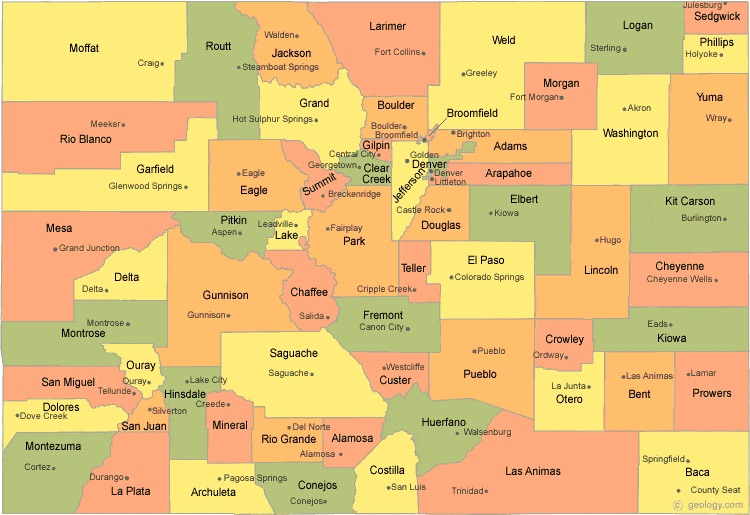
\includegraphics[width=0.4\textwidth]{images/CO_counties.jpg}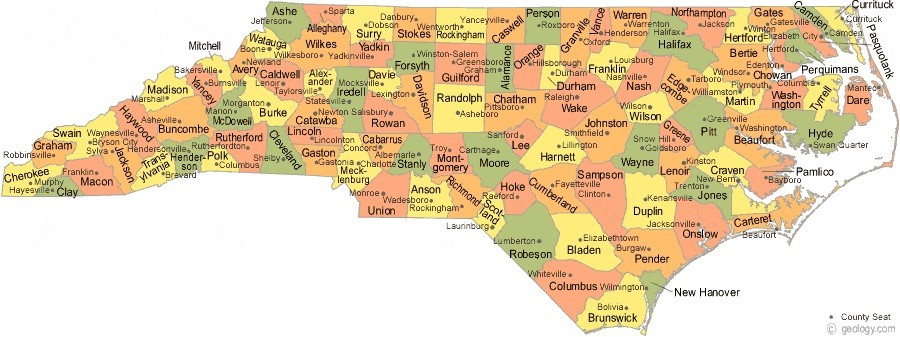
\includegraphics[width=0.4\textwidth]{images/NC_counties.jpg}\\
  \scriptsize{Colorado \hspace*{5cm} North Carolina}
\end{figure}

While they are kind of odd in terms of their heterogeneity, however, they are common units of analysis for US government data because they are more granular than states, but also big enough that reporting the number of deaths from drug overdoses in a given county doesn't threaten the privacy of individuals. And indeed, in this analysis, we will find that all our data is available at \emph{at least} the county level.

Things to know about counties:

\begin{itemize}
  \item There are about 3,200 counties in the United States.
  \item Counties vary dramatically in population and geographic size
  \item County names are \emph{not} unique across states. The same county name will appear in many states.
  \item Counties are sometimes called other things, like ``parish'' (in Louisiana), or occasionally ``borough''.
  \item All US counties and states have assigned numeric identifiers called ``FIPS codes.'' Not all datasets will include county's FIPS codes, but if you can find them, they're much easier to use than county names since you don't have to worry about capitalizations and such. You can find datasets online easily that will tell you the FIPS code for a given county given its state and name.
  \begin{itemize}
    \item County FIPS codes are often represented as the concatenation of a 2 digit State FIPS code and a 3 digit County FIPS Code. So if you are in the County of Autauga (County 1) in Alabama (State 1), you could see a county FIPS code of 01001, or you might see it broken out into a State FIPS code of 1, and a County FIPS code of 1. Sorry, just how it happens. :)
  \end{itemize}
  \item Just drop the state of Alaska (AK) from your analysis. It has some weird things going on with its county designations moving from before 2010 to after 2010, and they aren't worth dealing with.
\end{itemize}

\subsection*{Policy Changes}

In this analysis, we'll be analyzing \emph{three} policy changes:

\begin{itemize}

\item Florida, Effective February, 2010
\begin{itemize}
  \item \textbf{Changes:} ``Florida gained notoriety after 2007 because of the proliferation of pain clinics in the state that were prescribing large quantities of drugs for pain with little medical justification and were being used primarily by persons abusing or diverting opioid analgesics, benzodiazepines, and muscle relaxants. In 2010, Florida was also home to 98 of the 100 U. S. physicians who dispensed the highest quantities of oxycodone directly from their offices. In response, Florida enacted several measures to address prescribing that was inconsistent with best practices. The Florida legislature required that pain clinics treating pain with controlled substances register with the state by January 4, 2010. In February 2010, the Drug Enforcement Administration and various Florida law enforcement agencies began to work together in Operation Pill Nation. Pain clinic regulations were further expanded later in 2010. In February 2011, law enforcement conducted statewide raids, resulting in numerous arrests, seizures of assets, and pain clinic closures. In July of that year, coinciding with a public health emergency declaration by the Florida Surgeon General, the state legislature prohibited physician dispensing of schedule II or III drugs from their offices and activated regional strike forces to address the emergency. Mandatory dispenser reporting to the newly established prescription drug monitoring program began in September 2011. Finally, in 2012, the legislature expanded regulation of wholesale drug distributors and created the Statewide Task Force on Prescription Drug Abuse and Newborns.''\footnote{Source: Johnson, Paulozzi, Porucznik, Mack, and Herter, 2014.}
  \item \textbf{Note:} Obviously what we have here is a \emph{series} of changes rather than one single large change. Nevertheless, for this analysis just operationalize the policy change as having taken place in February 2010.
\end{itemize}
  \item Texas, Effective January 4, 2007
  \begin{itemize}
    \item \textbf{Changes:} ``In 2007, the Texas Medical Board adopted regulations with regards to treating pain with
controlled substances. The guidelines include performing a patient evaluation before prescribing opioids (including reviewing
prescription data and history related to the patient contained in the state’s prescription drug monitoring program (PDMP)), obtaining informed consent from the patient for opioid treatment, conduct periodic review of the opioid treatment, and maintain a complete medical record of the patient’s treatment.''\footnote{Source: The Network for Public Health Law, \href{https://azdhs.gov/documents/prevention/womens-childrens-health/injury-prevention/opioid-prevention/appendix-b-state-by-state-summary.pdf}{Appendix B}}. \href{https://texreg.sos.state.tx.us/public/readtac$ext.TacPage?sl=R&app=9&p_dir=&p_rloc=&p_tloc=&p_ploc=&pg=1&p_tac=&ti=22&pt=9&ch=170&rl=3}{Link to law.}
  \end{itemize}
  \item Washington (the State, not Washington, DC), Effective Jan 2, 2012.
  \begin{itemize}
    \item \textbf{Changes:} In 2011, the Washington Department of Health adopted a rule regulating the prescribing of opioids for pain treatment. Some of the prescribing requirements include:\footnote{Source: The Network for Public Health Law, \href{https://azdhs.gov/documents/prevention/womens-childrens-health/injury-prevention/opioid-prevention/appendix-b-state-by-state-summary.pdf}{Appendix B}}
    \begin{itemize}
      \item For patients who are stable involving non-escalating daily doses of 40 mg MED/day or less, periodic reviews shall take place annually.
      \item Mandatory consultation threshold for adults is 120 mg MED/day (oral).
      \item In the event a physician prescribes a dosage that meets or exceeds the consultation
      threshold, a consultation with a pain management specialist is required.
      \item The physician shall document each mandatory consultation.
      \item Recommended that a practitioner not prescribe more than an average of MED of
      120 mg without either the patient demonstrating improvement in function or without first obtaining a consultation from a pain management expert.
    \end{itemize}
    \item \href{http://apps.leg.wa.gov/documents/laws/wsr/2011/12/11-12-025.htm}{Link to regulation.}
    \end{itemize}
\end{itemize}


\subsection*{Your Task}

Your task is to complete both:

\begin{itemize}
  \item a pre-post analysis, and
  \item a difference-in-difference analysis
\end{itemize}

for all three of these policy changes. You can present your results in the graphical format modeled above. While there are many statistical methods of doing things like adding controls for various observable factors, the emphasis on this analysis is on data wrangling and transparent analysis, so those plots will be sufficient.

For the Florida case, you must analyze the effect of its policy change on \emph{BOTH} opioid shipments and overdose deaths.

For Texas and Washington, you only need to analyze overdose deaths. This is because our opioid shipment data only runs from 2006 to 2012, meaning that you only have one year of data on either side of the policy change, making evaluation of trends difficult. The overdose data I have provided, by contrast, runs from 2003-2015. With that said, \emph{any group that would like to analyze opioid shipment data \emph{by month} instead of by year for Texas and Washington (which would get you 12 observations with which to measure trends) would get extra credit for their project.}

For this project, you must:

\begin{itemize}
  \item Gather all data needed to complete this analysis
  \item Clean, organize, and merge it in order to allow for creation of the final analysis.
  \item Do all your work transparently through github \emph{as a team}.
  \begin{itemize}
    \item All team members must make substantial commits to the project.
    \item All team members must also actively review at least one PR for another team member. \textbf{You will be graded on your own code review. \emph{Your} code review is where YOU review the code of someone else, not where you have your code reviewed!}
  \end{itemize}
  \item Present \textbf{TWO} final reports, one for me, one for an imaginary policy maker (who is \emph{not} a statistician).
  \item In the report for me, include:
  \begin{itemize}
    \item The motivation for the project,
    \item The motivation for the research design being used,
    \item Details of the data used and how different datasets have been related to one another,
    \item Summary statistics for your data,
    \item Your analysis,
    \item Your interpretation of that analysis.
  \end{itemize}
  \item In the report for a policy maker (someone who is NOT trained in statistics), include:
  \begin{itemize}
    \item The motivation for the project,
    \item Overview of the data being used,
    \item Your analysis (presented for a non-statistician),
    \item Your \emph{interpretation} of that analysis (again, laying out strengths and weaknesses without using statistical jargon).
  \end{itemize}
\end{itemize}


In writing your report, remember that much of the focus of this project is on \emph{data wrangling}, so spend lots of time on your data section for me discussing where you data came from, what assumptions you've made in working with it, and how you handled issues you ran into.

\subsection*{Due Dates}
\begin{itemize}
  \item An outline of your project strategy is due on October 22nd.
  \begin{itemize}
    \item In writing this strategy, use a ``backwards design'' organizational scheme (we'll discuss these much more in the future, but for now you get to explore yourself!): Start by establishing what you want to achieve (i.e. the plots I've already specified). Then ask: What dataset do I need to make these plots? Or more specifically:
    \begin{itemize}
      \item What variables will I need in this data?
      \item What sample (what years, what counties, etc.) needs to be covered in this data?
      \item What should a single row of this data look like (i.e. what's a unit of observation?)
    \end{itemize}
    \item Then step back and repeat the process: to get this dataset, what do I need to do? What do I need my input datasets to look like to get to this final analysis dataset?
    \item Then again: to get to these intermediate datasets, what source datasets do I need? What variables do they need?
    \item Then start trying to assign the tasks implied by that analysis to people. (OBVIOUSLY this will only be very approximate!! But it's good to think about this before you start, then adapt as you move forward).
  \end{itemize}
  This should include a summary of the datasets you plan to use, a summary of how you plan to merge these datasets, who will be responsible for writing initial code for each step, and who will review each set of code.
  \item A preliminary draft of your report will be due November 5th.
  \item A final draft of your report will be due November 19th.
\end{itemize}

\subsection*{Tips}
\begin{itemize}
  \item Keep your \emph{source} datasets in a common dropbox folder. You should \emph{only} ever read data from your source data, not modify it directly. This is to ensure that your source files never get corrupted. Because of that, it's fine to have it live outside your github repo.
  \item Store your intermediate files (the results of reading data from the source files and making modifications) in your repository using git-lfs. Store the files in \texttt{parquet} format with to minimize memory use.
\end{itemize}

\appendix

\section{Difference-in-difference Regressions}\label{appendix_diffindiff}

of the following form (where $c$ is an index for US Counties (a geographic unit of observation within states), and $t$ is an index for time):

\emph{Allowing only for level changes:}
\begin{eqnarray}
 Y_{c,t} &=& \alpha + \psi_{c} + \beta_1 post_{t} + \label{diff_in_diff_notime}\\
  && \beta_2 post_{t} * policy\_state_{c} + \epsilon_{c,t} \nonumber
\end{eqnarray}

Where $Y_{c,t}$ is a county-year-level outcome (either overdoses per capita or opioid shipments),  $\psi_c$ are county fixed effects, $post_{t}$ is an indicator for whether we are in a period after implementation of the policy change, and $policy\_state_{c}$ is an indicator for whether a given county is in a state that experienced a policy change. Our ``difference-in-difference'' estimate is the coefficient $\beta_2$.

However, note that the analysis in Figure~\ref{figure_diffindiff_examples} allows for time trends, which do not appear in this specification \ref{diff_in_diff_notime}. It just compares differences in average levels of overdoses before and after the policy change. If we also want to allow for differential time trends (as pictured above) we'd use specification \ref{diff_in_diff_wtime}:

\emph{Allowing for both changes in levels and for changes in trends (analogous to what we plotted above):}
\begin{eqnarray}
 Y_{c,t} &=& \alpha + \label{diff_in_diff_wtime}\\
 && \beta_1 policy\_state_{c} + \nonumber\\
 && \beta_2 year_{t} + \beta_3 year * policy\_state_{c} + \nonumber\\
 && \beta_4 post_{t} + \beta_5 post_{t} * policy\_state_{t} + \nonumber \\
 && \beta_6 post_{t} * year + \nonumber\\
 && \beta_7 post_{t} * year_{t} * policy\_state_{c} + \epsilon_{c,t} \nonumber
\end{eqnarray}

Where $year_{t}$ has been adjusted to take on a value of 0 at the year of the policy change.


We can interpret these as follows, where for simplicity I'll just call our policy-change state ``Treated,'' and non-policy change states as ``Controls.''

\begin{itemize}
  \item $\alpha$ is the intercept for the Controls in the pre-policy change period (note that the intercept occurs at the year of the policy chance, since that's where $t=0$).
  $\alpha + \beta_{1}$ is the intercept for Treated in the pre-policy change period.
  \begin{itemize}
    \item Consequently, $\beta_1$ is the \emph{difference} in intercepts at $t=0$ for the pre-policy change period.
  \end{itemize}
  \item $\alpha + \beta_4$ is the intercept for the Controls in the pre-policy change period. $\alpha + \beta_1 + \beta_4 + \beta_5$ is the intercept for Treated in the pre-policy change period.
  \begin{itemize}
    \item Consequently, $\beta_1 + \beta_5$ is the \emph{difference} in intercepts at $t=0$ for the post-policy change period.
  \end{itemize}
  \item $\beta_2$ is the slope for Controls before the policy change. $\beta_2 + \beta_3$ is the slope for Treated before the policy change.
\begin{itemize}
  \item Consequently, $\beta_{3}$ is the \emph{difference} in slopes in the pre-policy change period.
\end{itemize}
  \item $\beta_{2} + \beta_{6}$ is the slope in the post-policy change period for Control states. $\beta_{2} + \beta_{3} + \beta_{6} + \beta_{7}$ is the slope for Treated in the post-change period.
  \begin{itemize}
    \item Consequently, $\beta_{3} + \beta_{7}$ is the difference in slopes in the post-policy change period.
  \end{itemize}
  \item The \emph{difference-in-difference} estimate for the change in intercepts is therefore: \\
   $(\beta_1 + \beta_5) - (\beta_1) = \beta_5$
  \item The \emph{difference-in-difference} estimate for the change in slopes is therefore:\\
   $(\beta_{3} + \beta_{7}) - (\beta_{3}) = \beta_7$.
\end{itemize}

So far so good! But we are often interested in asking about how things look \emph{on the whole} at some point after a policy has changed, not right at the moment of the policy change.

This is also helpful in situations where level shifts go one way (say, seem to make stuff worse), but the slope change goes the other (seems to make stuff better). At what point do those offset? After 2 years, for example, is everyone better off?

These quantities are quite tricky because you have to estimate them \emph{at a point in time}, which means bringing in specific values of $t$. (Again: this is after we've normalized $year$ so that $t=0$ occurs at the year of the policy change. )

Suppose, for example, we wanted to compare outcomes 2 years after the policy to 1 year before the policy change. Here are the predicted values (note how we now have to fill in values for $year$'):

\begin{itemize}
  \item Treated at 2 years after policy change: \\
  $\alpha + \beta_1 + \beta_2 * 2 + \beta_3 * 2 + \beta_4 + \beta_5 + \beta_6 * 2 + \beta_7 * 2$
  \item Control at 2 years after policy change: \\
  $\alpha + \beta_2 * 2 + \beta_4 + \beta_6 * 2$
  \item Treated 1 year before policy change: \\
  $\alpha + \beta_1 + \beta_2 * -1 + \beta_3 * -1$
  \item Control 1 year before policy change: \\
  $\alpha + \beta_2 * -1$
\end{itemize}

Now differencing:

\begin{itemize}
  \item Difference (T - C) two years out: \\
  $\beta_1  + \beta_3 * 2+ \beta_5 + \beta_7 * 2$
  \item Difference (T-C) one year before: \\
  $\beta_1  + \beta_3 * -1$
  \item Difference-in-difference from two years after minus one year before: \\
  $\beta_7 * 2 + \beta_5 + \beta_3$
\end{itemize}

Yeah... see? That doesn't just drop out of the regression table, and nor does an estimate of significance. And that's why we use post-regression tests!

\subsection*{Fixed-Effects}

It is also normal to do the difference-in-difference regression described above with fixed-effects. Note, however, that this changes the specification somewhat because $policy\_state_{c}$ is non-time-varying,  and so will be co-linear with county fixed effects, and so it won't be possible to estimate it. That doesn't change the diff-in-diff estimates, but it does make reading the equations a little trickier, so I did the writeup above without fixed effects. In general, though, its best to use fixed effects when you can!




\end{document}
